%straight line split with right angle
\documentclass[tikz,border=10pt]{standalone}
\usepackage{tikz}
\usetikzlibrary{angles,quotes,calc} % Add this for angle labels

\begin{document}

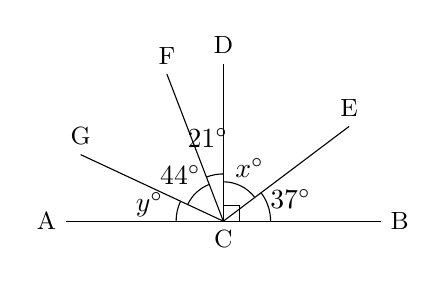
\begin{tikzpicture}[scale=1]
    % Define the points of the cube
    \coordinate (A) at (0,0);
    \coordinate (B) at (4,0);
    \coordinate (C) at (2,0);
    \coordinate (D) at (2,2);
    \coordinate (E) at ($(C)+(37:2cm)$); 
    \coordinate (F) at ($(C)+(111:2cm)$); 
    \coordinate (G) at ($(C)+(155:2cm)$); 

    % Draw the visible edges of the cube
    \draw (A) -- (B);
    \draw (C) -- (D);
    \draw (C) -- (F);
    \draw (C) -- (G);
    \draw (C) -- (E);

    % Draw the right angle
    \draw (C) ++(0:0.2) -- ++(90:0.2) -- +(180:0.2);
    
    % Draw the angle between lines
    \pic [draw, "$37^{\circ}$", angle eccentricity=1.5, angle radius=0.6cm] {angle = B--C--E};
    \pic [draw, "$x^{\circ}$", angle eccentricity=1.5, angle radius=0.5cm] {angle = E--C--D};
    \pic [draw, "$21^{\circ}$", angle eccentricity=1.8, angle radius=0.6cm] {angle = D--C--F};
    \pic [draw, "$44^{\circ}$", angle eccentricity=1.6, angle radius=0.5cm] {angle = F--C--G};
    \pic [draw, "$y^{\circ}$", angle eccentricity=1.6, angle radius=0.6cm] {angle = G--C--A};

    % Place the labels with smaller font size
    \node at (A) [left,font=\small] {A};
    \node at (B) [right,font=\small] {B};
    \node at (C) [below,font=\small] {C};
    \node at (D) [above,font=\small] {D};
    \node at (E) [above,font=\small] {E};
    \node at (F) [above,font=\small] {F};
    \node at (G) [above,font=\small] {G};
    
\end{tikzpicture}

\end{document}